\let\negmedspace\undefined
\let\negthickspace\undefined
\documentclass[journal]{IEEEtran}
\usepackage[a5paper, margin=10mm, onecolumn]{geometry}
%\usepackage{lmodern} % Ensure lmodern is loaded for pdflatex
\usepackage{tfrupee} % Include tfrupee package

\setlength{\headheight}{1cm} % Set the height of the header box
\setlength{\headsep}{0mm}     % Set the distance between the header box and the top of the text

\usepackage{gvv-book}
\usepackage{gvv}
\usepackage{cite}
\usepackage{amsmath,amssymb,amsfonts,amsthm}
\usepackage{algorithmic}
\usepackage{graphicx}
\usepackage[compatibility=false]{caption}
\usepackage{textcomp}
\usepackage{xcolor}
\usepackage{txfonts}
\usepackage{listings}
\usepackage{enumitem}
\usepackage{mathtools}
\usepackage{gensymb}
\usepackage{comment}
\usepackage[breaklinks=true]{hyperref}
\usepackage{tkz-euclide} 
\usepackage{listings}
% \usepackage{gvv}                                        
\def\inputGnumericTable{}                                 
\usepackage[latin1]{inputenc}                                
\usepackage{color}                                            
\usepackage{array}                                            
\usepackage{longtable}                                       
\usepackage{calc}                                             
\usepackage{multirow} 
\usepackage{hhline}                                           
\usepackage{ifthen}                                           
\usepackage{lscape}
\usepackage{circuitikz}
\tikzstyle{block} = [rectangle, draw, fill=blue!20, 
    text width=4em, text centered, rounded corners, minimum height=3em]
\tikzstyle{sum} = [draw, fill=blue!10, circle, minimum size=1cm, node distance=1.5cm]
\tikzstyle{input} = [coordinate]
\tikzstyle{output} = [coordinate]

\begin{document}
\bibliographystyle{IEEEtran}
\vspace{3cm}

\title{MatGeo Assignment 9.2.41}
\author{AI25BTECH11007}
 \maketitle
% \newpage
% \bigskip
{\let\newpage\relax\maketitle}

\renewcommand{\thefigure}{\theenumi}
\renewcommand{\thetable}{\theenumi}
\setlength{\intextsep}{10pt} % Space between text and floats


\numberwithin{equation}{enumi}
\numberwithin{figure}{enumi}
\renewcommand{\thetable}{\theenumi}
\noindent
\textbf{Question :}\\
 Find the area of the region bounded by the curves $y^2$ = 9x, y = 3x.
 
\noindent\\
\textbf{Solution :}\\ 
\begin{align}
  \text{Given curves: } 
  & y^2 = 9x, \quad y = 3x
\end{align}
The conic can be written as
\begin{align}
g(\vec{x}) = \vec{x}^T\vec{V}\vec{x} + 2\vec{u}^T\vec{x} + f = 0
\end{align}
where
\begin{align}
\vec{V} = \myvec{0 & 0 \\ 0 & 1}, \quad
\vec{u} = \myvec{-\tfrac{9}{2} \\ 0}, \quad
f = 0
\end{align}

The equation of the line is
\begin{align}
\vec{x} = \vec{h} + \kappa \vec{m}
\end{align}
where
\begin{align}
\vec{h} = \myvec{0 \\ 0}, \quad 
\vec{m} = \myvec{1 \\ 3}
\end{align}

Substituting in $g(\vec{x}) = 0$:
\begin{align}
(\vec{h} + \kappa\vec{m})^T\vec{V}(\vec{h} + \kappa\vec{m})
+ 2\vec{u}^T(\vec{h} + \kappa\vec{m}) + f = 0
\end{align}

Expanding,
\begin{align}
\kappa^2 (\vec{m}^T\vec{V}\vec{m}) + 2\kappa(\vec{m}^T(\vec{V}\vec{h} + \vec{u})) + (\vec{h}^T\vec{V}\vec{h} + 2\vec{u}^T\vec{h} + f) = 0
\end{align}

Substituting the known values,
\begin{align}
9\kappa^2 - 9\kappa = 0
\end{align}
\[
\kappa_1 = 0, \quad \kappa_2 = 1
\]

\noindent
Finally, intersecting points are
\begin{align}
\vec{x}_1 &= \myvec{0 \\ 0} + 0\myvec{1 \\ 3} = \myvec{0 \\ 0} \\[2mm]
\vec{x}_2 &= \myvec{0 \\ 0} + 1\myvec{1 \\ 3} = \myvec{1 \\ 3}
\end{align}

\noindent
Thus, the points of intersection are 
\[
A = \myvec{0 \\ 0}, \quad B = \myvec{1 \\ 3}
\]
 
Hence, the required area is
\begin{align}
A &= \int_{0}^{1} (3\sqrt{x} - 3x)\,dx \\[2mm]
\end{align}
\[
\boxed{A = \tfrac{1}{2} \text{ square units}}
\]

\begin{figure}[H]
    \centering
    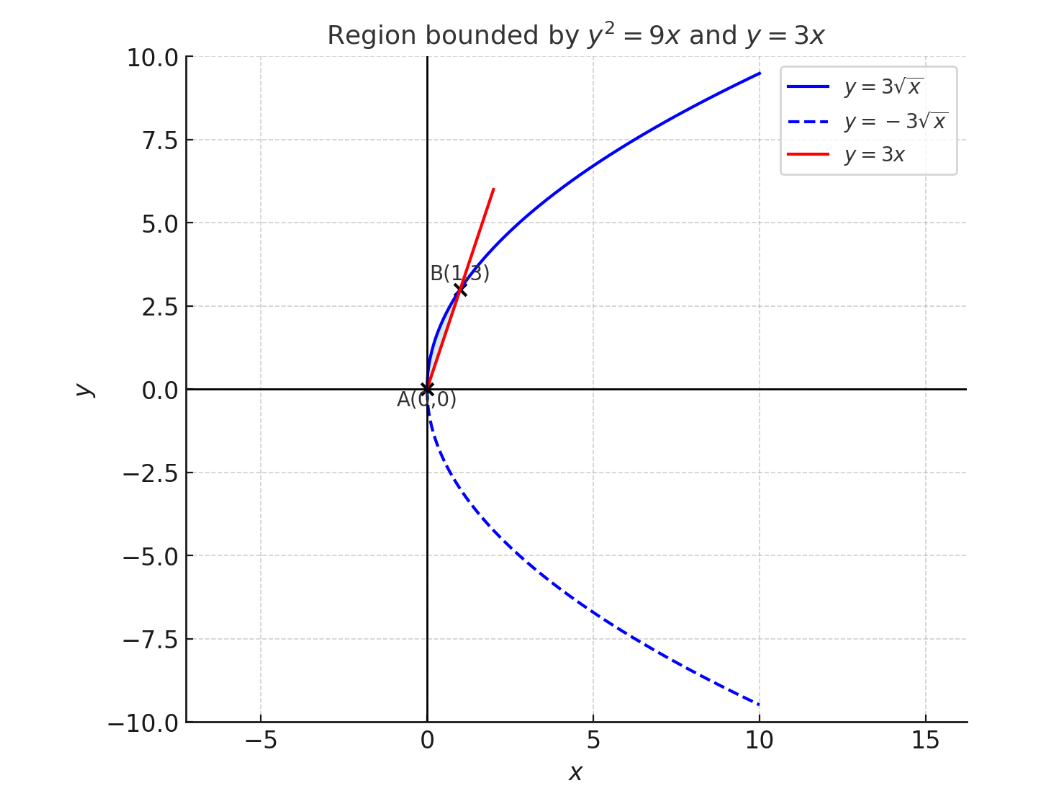
\includegraphics[width=0.85\linewidth]{figs/image.png}
    \caption{Image}
    \label{fig:placeholder}
\end{figure}

\end{document}